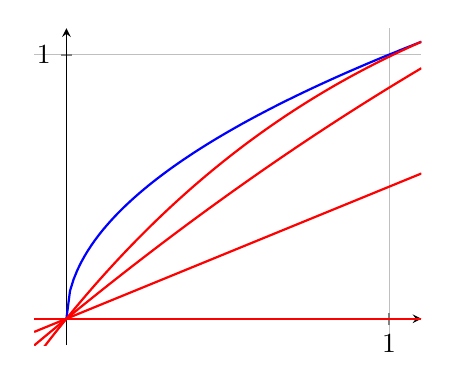
\begin{tikzpicture}
    \begin{axis}[width=6.5cm,
        axis lines=middle,
        grid=major,
        xmin=-0.1, xmax=1.1,
        ymin=-0.1, ymax=1.1,
        % xlabel=$x$, xlabel style={right},
        % ylabel=$y$, ylabel style={above},
        tick style={thick},
        ticklabel style={font=\normalsize},
        xtick={0, 1}, 
        ytick={0, 1},
        % legend entries={0.5x},
            legend style={
            at={(1.05,0.4)},
            anchor=north,
            legend columns=1},
            legend cell align={left}
    ]
    
    \def\a{-0.1}
    \def\b{1.1}
    
    \addplot[blue,thick,samples=100,domain=0:\b] {x^(1/2)};
    \addplot[red,thick,samples=100,domain=\a:\b] {0};
    \addplot[red,thick,samples=100,domain=\a:\b] {x/2};
    \addplot[red,thick,samples=100,domain=\a:\b] {-1/8*x^2+x};
    \addplot[red,thick,samples=100,domain=\a:\b] {-1/128*x^4+1/8*x^3-5/8*x^2+3/2*x};
    \end{axis}
\end{tikzpicture}


%import matplotlib.pyplot as plt
%import numpy as np
%from numpy.polynomial import Polynomial

%PAS = 1e-3
%n = 8
%X = np.arange(0, 1, PAS)


%P = Polynomial([0])
%plt.plot(X, P(X))

%for k in range(n):
%    P = P + 1/2 * (Polynomial([0, 1]) - P ** 2)
%    plt.plot(X, P(X))

%racine = [np.sqrt(x) for x in X]
%plt.plot(X, racine, 'r')
%plt.show()
